\documentclass[11pt,oneside]{article}	%use"amsart"insteadof"article"forAMSLaTeXformat
\usepackage{geometry}		%Seegeometry.pdftolearnthelayoutoptions.Therearelots.
\geometry{letterpaper}		%...ora4paperora5paperor...
%\geometry{landscape}		%Activateforforrotatedpagegeometry
%\usepackage[parfill]{parskip}		%Activatetobeginparagraphswithanemptylineratherthananindent
\usepackage{graphicx}				%Usepdf,png,jpg,orepsßwithpdflatex;useepsinDVImode
								%TeXwillautomaticallyconverteps-->pdfinpdflatex		
\usepackage{amssymb}
\usepackage{hyperref}

\usepackage{framed}
\usepackage{amsthm}
\newtheorem{remark}{Remark}
\newtheorem{definition}{Definition}

%----macros begin---------------------------------------------------------------
\usepackage{color}
\usepackage{amsthm}

\def\conv{\mbox{\textrm{conv}\,}}
\def\aff{\mbox{\textrm{aff}\,}}
\def\E{\mathbb{E}}
\def\R{\mathbb{R}}
\def\Z{\mathbb{Z}}
\def\tex{\TeX}
\def\latex{\LaTeX}
\def\v#1{{\bf #1}}
\def\p#1{{\bf #1}}
\def\T#1{{\bf #1}}

\def\vet#1{{\left(\begin{array}{cccccccccccccccccccc}#1\end{array}\right)}}
\def\mat#1{{\left(\begin{array}{cccccccccccccccccccc}#1\end{array}\right)}}

\def\lin{\mbox{\rm lin}\,}
\def\aff{\mbox{\rm aff}\,}
\def\pos{\mbox{\rm pos}\,}
\def\cone{\mbox{\rm cone}\,}
\def\conv{\mbox{\rm conv}\,}
\newcommand{\homog}[0]{\mbox{\rm homog}\,}
\newcommand{\relint}[0]{\mbox{\rm relint}\,}

%----macros end-----------------------------------------------------------------

\title{Imaging Morphology with LAR
\footnote{This document is part of the \emph{Linear Algebraic Representation with CoChains} (LAR-CC) framework~\cite{cclar-proj:2013:00}. \today}
}
\author{Alberto Paoluzzi}
%\date{}							%Activatetodisplayagivendateornodate

\begin{document}
\maketitle
\nonstopmode

\begin{abstract}
In this module we aim to implement the four operators of mathematical morphology, i.e.~the \emph{dilation}, \emph{erosion}, \emph{opening} and \emph{closing} operators, by the way of matrix operations representing the linear operators---\emph{boundary} and \emph{coboundary}---over LAR. 
According to the multidimensional character of LAR, our implementation is dimension-independent.
In few words, it works as follows: (a)  the input is (the coordinate representation of) a $d$-chain $\gamma$; (b) compute its boundary $\partial_d(\gamma)$; (c) extract the maximal $(d-2)$-chain $\epsilon \subset \partial_d(\gamma)$; (d) consider the $(d-1)$-chain returned from its coboundary $\delta_{d-2}(\epsilon)$; (e) compute the $d$-chain $\eta := \delta_{d-1}(\delta_{d-2}(\epsilon)) \subset C_d$ \emph{without} performing the  $\mbox{mod\ 2}$ final transformation on the resulting coordinate vector, that would provide a zero result, according to the standard algebraic constraint $\delta\circ\delta=0$. It is easy to show that $\eta \equiv (\oplus \gamma) - (\ominus \gamma)$ provides the \emph{morphological gradient} operator. The four standard morphological operators are therefore  consequently computable.
\end{abstract}

\tableofcontents

\section{Test image generation}

Various methods for the input or the generation of a test image  are developed in the subsections of this section. The aim is to prepare a set of controlled test beds, used to check both the implementation and the working properties of our topological implementation of morphological operators. 


\subsection{Random binary multidimensional image}

A multidimensional binary image is generated here by using a random approach, both for the bulk structure and the small artefacts of the image.  


%-------------------------------------------------------------------------------
@d Generation of random image
@{def randomImage(shape, structure, noiseFraction=0.1):
	""" Generation of random image of given shape and structure. 
		Return a scipy.ndarray(shape)
	"""
	rows, columns = shape
	rowSize, columnSize = structure						
	random_array = randint(0, 255, size=(rowSize, columnSize))
	image_array = numpy.zeros((rows, columns))
	@< Generation of bulk array structure @>
	@< Generation of random artifacts @>
	return image_array
@}
%-------------------------------------------------------------------------------


\paragraph{Generation of the gross image}
First we generate a 2D grid of squares by Cartesian product, and produce the bulk of the random image then used to test our approach to morphological operators via topological ones.


%import scipy
%scipy.misc.imsave('outfile.jpg', image_array)
%
%scipy.ndimage.imread(fname, flatten=False, mode=None)[source]
%
%rand(10, 10)
%
	
%-------------------------------------------------------------------------------
@d Generation of bulk array structure
@{for i in range(rowSize):
	for j in range(columnSize):
		for h in range(i*rowSize,i*rowSize+rowSize): 
			for k in range(j*columnSize,j*columnSize+columnSize):
				if random_array[i,j] < 127:
					image_array[h,k] = 0 
				else: 
					image_array[h,k] = 255
@}
%-------------------------------------------------------------------------------

\paragraph{Generation of random artefacts upon the image}

Then random noise is added to the previously generated image, in order to produce artifacts at the pixel scale. 

%-------------------------------------------------------------------------------
@d Generation of random artifacts
@{noiseQuantity = rows*columns*noiseFraction
k = 0
while k < noiseQuantity:
	i,j = randint(rows),randint(columns)
	if image_array[i,j] == 0: image_array[i,j] = 255
	else: image_array[i,j] = 0
	k += 1
scipy.misc.imsave('./outfile.png', image_array)
@}
%-------------------------------------------------------------------------------


\section{Selection of an image segment}

In this section we implement several methods for image segmentation and segment selection. 

\subsection{Selection of a test chain}

The first and simplest method is the selection of the portion of a binary image contained within a masking window.
Here we select the (white) sub-image contained in a given window, and compute the coordinate representation of the (chain) sub-image.

\paragraph{Mask definition}

A \emph{window} within a $d$-image is defined by $2\times d$ integer numbers (2 multi-indices), corresponding to the window  \texttt{minPoint} (minimum indices) and to the window \texttt{maxPoint} (maximum indices). A list of multi-index tuples, contained in the \texttt{window} variable, is generated by the function \texttt{setMaskWindow} below.

%-------------------------------------------------------------------------------
@d Generation of a masking window
@{def setMaskWindow(window,image_array):
	minPoint, maxPoint = window
	imageShape = list(image_array.shape)
	@< Generation of multi-index window @>
	@< Window-to-chain mapping @>
	@< Change chain color to grey @>
	return segmentChain
@}
%-------------------------------------------------------------------------------

The set of tuples of indices contained in a (multidimensional) window is given below.
 
%-------------------------------------------------------------------------------
@d Generation of multi-index window
@{indexRanges = zip(minPoint,maxPoint)
tuples = CART([range(min,max) for min,max in indexRanges])
@}
%-------------------------------------------------------------------------------



\subsection{Mapping of integer tuples to integers}

In order to produce the coordinate representation of a chain in a multidimensional image (or $d$-image) we need: (a) to choose a basis of image elements, i.e.~of $d$-cells, and in particular to fix an ordering of them; (b) to map the multidimensional index, selecting a single $d$-cell of the image, to a single integer mapping the cell to its linear position within the chosen basis ordering. 


\paragraph{Grid of hyper-cubes of unit size}
Let $S_i=(0,1,...,n_i-1)$ be ordered integer sets with $n_i$ elements, and 
\[
S= S_0 \times S_1 \times \cdots \times S_{d-1}
\] 
the set of indices of elements of a $d$-image.

\begin{definition}[$d$-image shape]
The \emph{shape} of a $d$-image with $n_0\times n_1 \times\cdots\times n_{d-1}$ elements (here called \emph{voxels}) is the ordered set $(n_0, n_1, \ldots, n_{d-1})$.
\end{definition}


\paragraph{$d$-dimensional row-major order}

Given a $d$-image with shape $S=(n_0,n_1,...,n_{d-1})$ and number of elements $n=\prod n_i$, 
the mapping  
\[
S_0 \times S_1 \times \cdots \times S_{d-1} \to \{ 0, 1, \ldots, n-1\}
\]
 is a {linear combination} with integer {weights}  $(w_0,w_1,...,w_{d-2},1)$, such that:
\[
(i_0,i_1,...,i_{d-1}) \mapsto i_0 w_0 +i_1 w_1 +\cdots +i_{d-1} w_{d-1},
\]
where 
\[
w_k = n_{k+1}  n_{k+2} \cdots  n_{d-1}, \qquad 0\leq k\leq d-2.
\]

\paragraph{From tuples multi-indices to chain coordinates}

The set of \texttt{tuples} of all pixels (or $d$-dimensional image elements) within the \emph{mask} is here mapped to the corresponding set of (single) integers associated to the low-level image elements (pixels or voxels, depending on the image dimension and shape), denoted \texttt{windowChain}. Such total chain of the mask \texttt{window} is then filtered to contain the only coordinates of \emph{white} image elements within the window, and returned as the set of integer cell indices \texttt{segmentChain}.

%-------------------------------------------------------------------------------
@d Window-to-chain mapping
@{d = len(imageShape)
weights = [PROD(imageShape[(k+1):]) for k in range(d-1)]+[1]
imageCochain = image_array.reshape(PROD(imageShape))
windowChain = [INNERPROD([index,weights]) for index in tuples]
segmentChain = [cell for cell in windowChain if imageCochain[cell]==255]
@}
%-------------------------------------------------------------------------------

\subsection{Show segment chain from binary image}

Now we need to show visually the selected \texttt{segmentChain}, by change the color of its cells from white (255) to middle grey (127). Just remember that \texttt{imageCochain} is the linear representation of the image, with number of cells equal to \texttt{PROD(imageShape)}. Then the modified image is restored within \texttt{image\_array}, and is finally exported to a \texttt{.png} image file.

%-------------------------------------------------------------------------------
@d Change chain color to grey
@{for cell in segmentChain: imageCochain[cell] = 127
image_array = imageCochain.reshape(imageShape)
scipy.misc.imsave('./outfile.png', image_array)
@}
%-------------------------------------------------------------------------------


\section{Construction of (co)boundary operators}

A $d$-image is a \emph{cellular $d$-complex} where cells are $k$-cuboids ($0\leq k\leq d$), i.e.~Cartesian products of a number $k$ of 1D intervals, embedded in $d$-dimensional Euclidean space. 

A direct construction of cuboidal complexes is offered in \texttt{larcc} by the \texttt{largrid} module. 
The \texttt{visImageChain} function given by the macro \emph{Visualisation of an image chain} below. 


\subsection{Visualisation of an image chain}

\paragraph{$d$-Chain visualisation}

%-------------------------------------------------------------------------------
@d Pyplasm visualisation of an image chain
@{def visImageChain (shape,chain):
	imageShape = list(shape)
	model = larCuboids(imageShape)
	imageVerts = model[0]
	imageLAR = model[1]
	chainLAR = [cell for k,cell in enumerate(imageLAR) if k in chain]
	return imageVerts,chainLAR
@}
%-------------------------------------------------------------------------------

\paragraph{Boundary visualisation of a $d$-chain}

%-------------------------------------------------------------------------------
@d Boundary visualisation of an image chain
@{def visImageChainBoundary (shape,chain):
	imageShape = list(shape)
	model = larCuboids(imageShape)
	imageVerts = model[0]
	skeletons = gridSkeletons(imageShape)
	facets = skeletons[-2]
	csrBoundaryMat = gridBoundaryMatrices(imageShape)[-1]
	csrChain = scipy.sparse.csr_matrix((PROD(imageShape),1))
	for k in chain: csrChain[k,0] = 1
	csrBoundaryChain = matrixProduct(csrBoundaryMat, csrChain)
	for k,value in enumerate(csrBoundaryChain.data):
		if MOD([value,2]) == 0: csrBoundaryChain.data[k] = 0
	cooBoundaryChain = csrBoundaryChain.tocoo()
	boundaryCells = [cooBoundaryChain.row[k] 
		for k,val in enumerate(cooBoundaryChain.data) if val == 1]
	return imageVerts,[facets[k] for k in boundaryCells]
@}
%-------------------------------------------------------------------------------

\begin{figure}[htbp] %  figure placement: here, top, bottom, or page
   \centering
   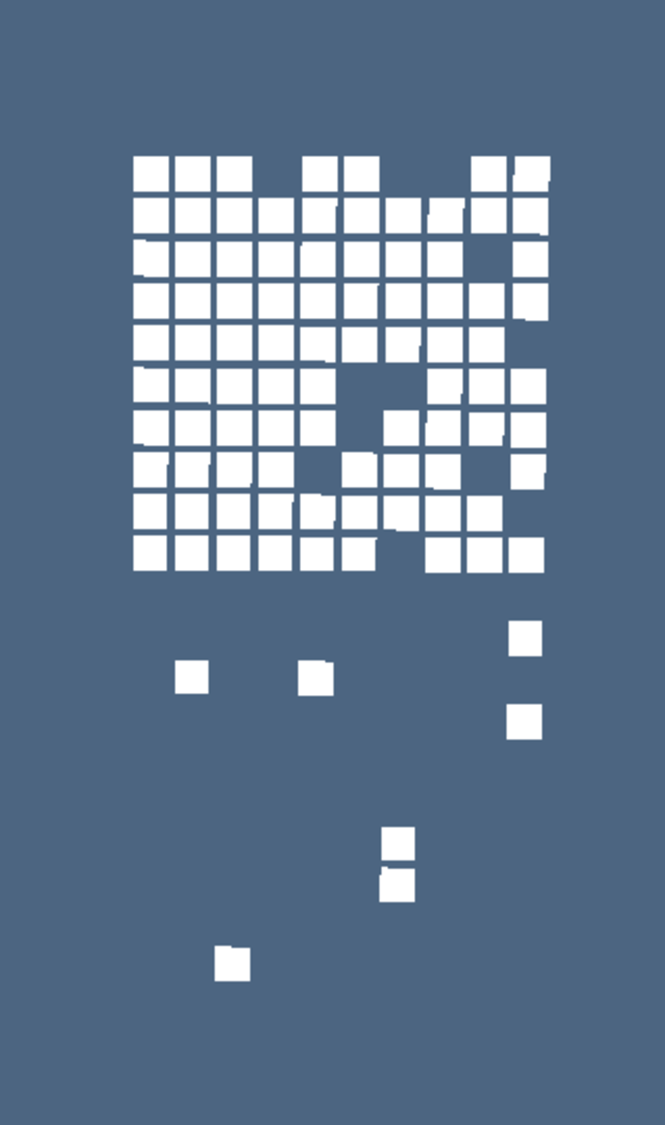
\includegraphics[height=0.3\linewidth,width=0.16\linewidth]{images/morph-chain2D1} 
   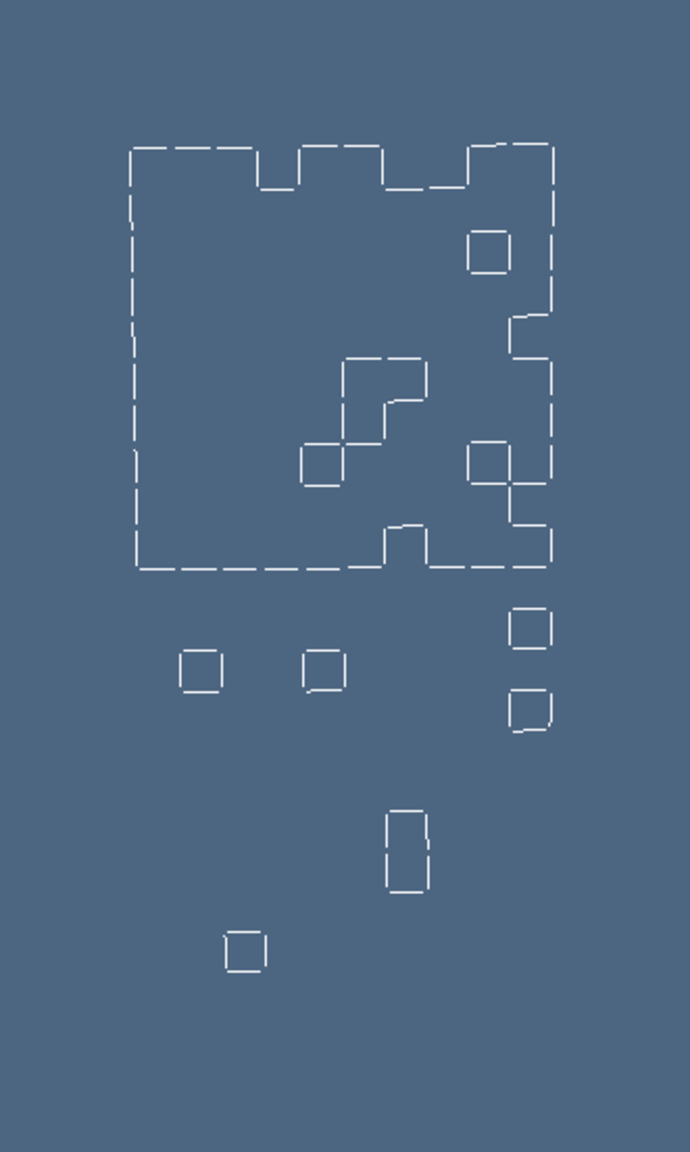
\includegraphics[height=0.3\linewidth,width=0.16\linewidth]{images/morph-chain1D1} 
   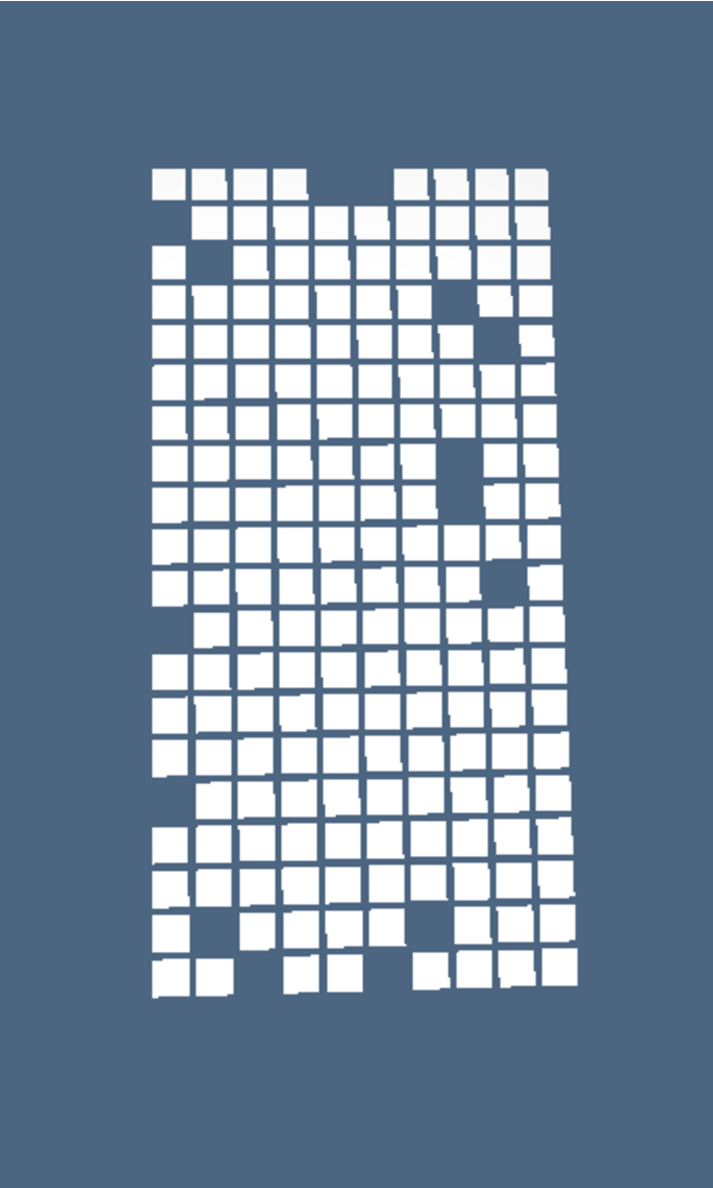
\includegraphics[height=0.3\linewidth,width=0.16\linewidth]{images/morph-chain2D2} 
   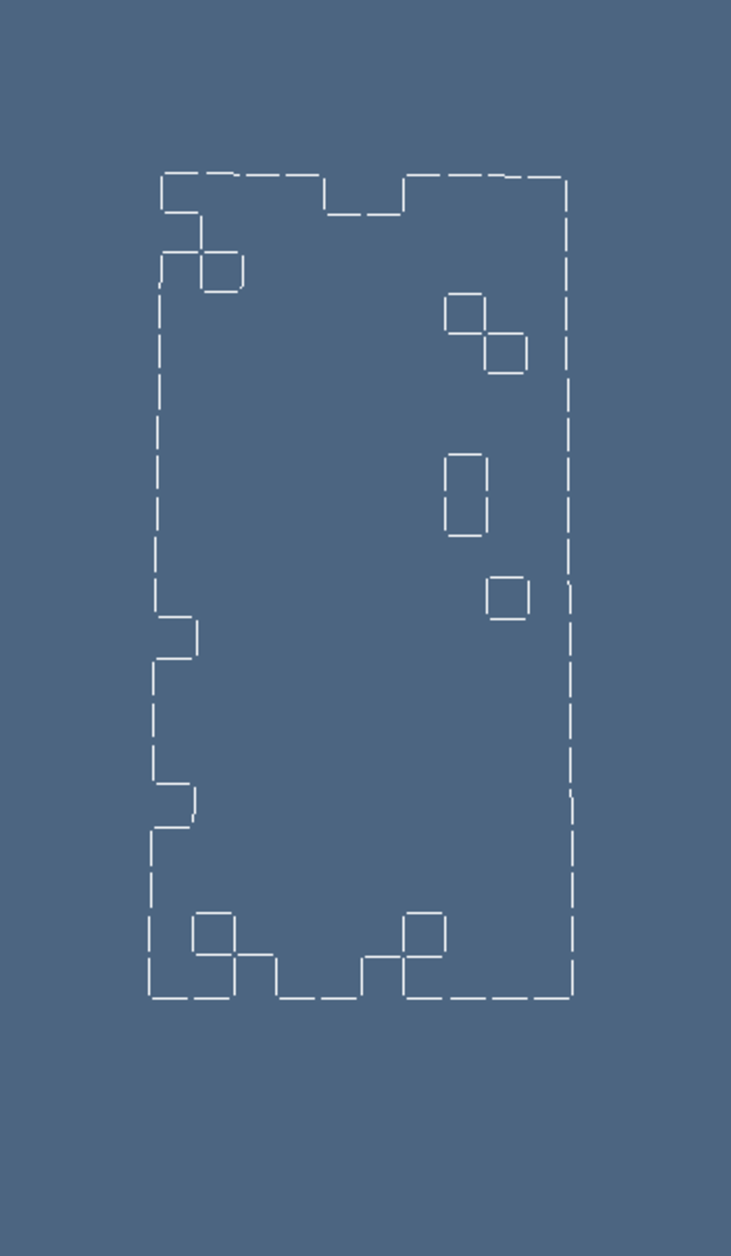
\includegraphics[height=0.3\linewidth,width=0.16\linewidth]{images/morph-chain1D2} 
   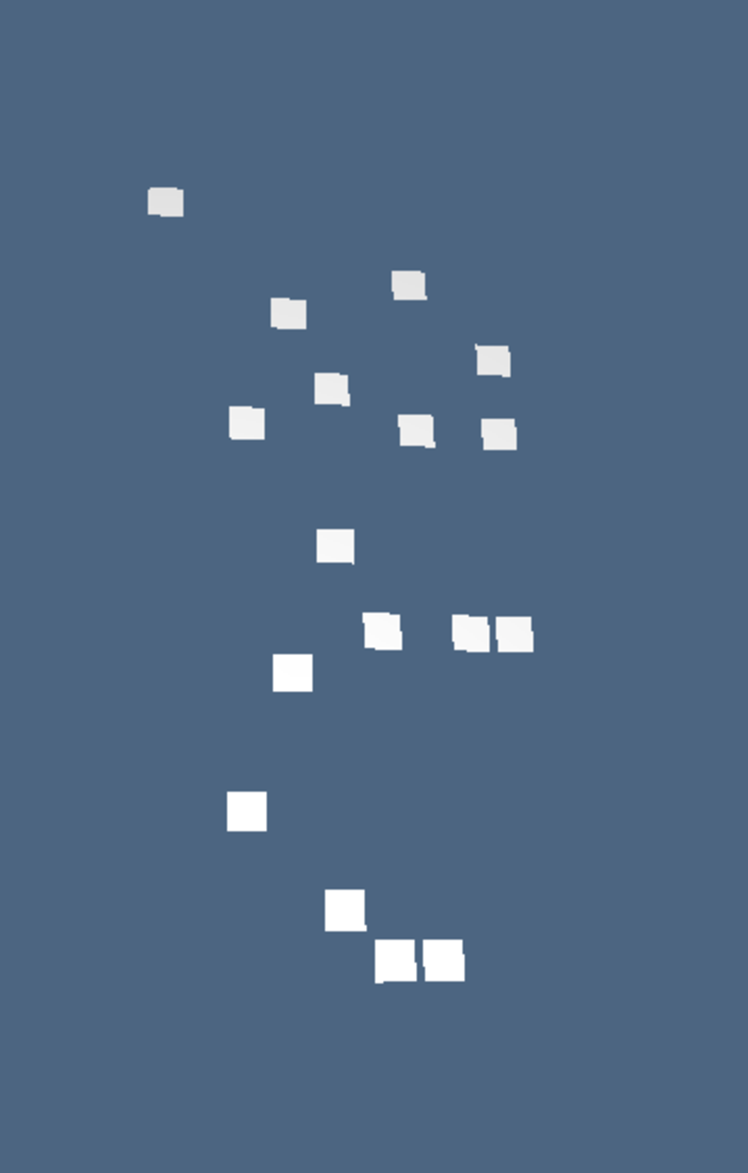
\includegraphics[height=0.3\linewidth,width=0.16\linewidth]{images/morph-chain2D3} 
   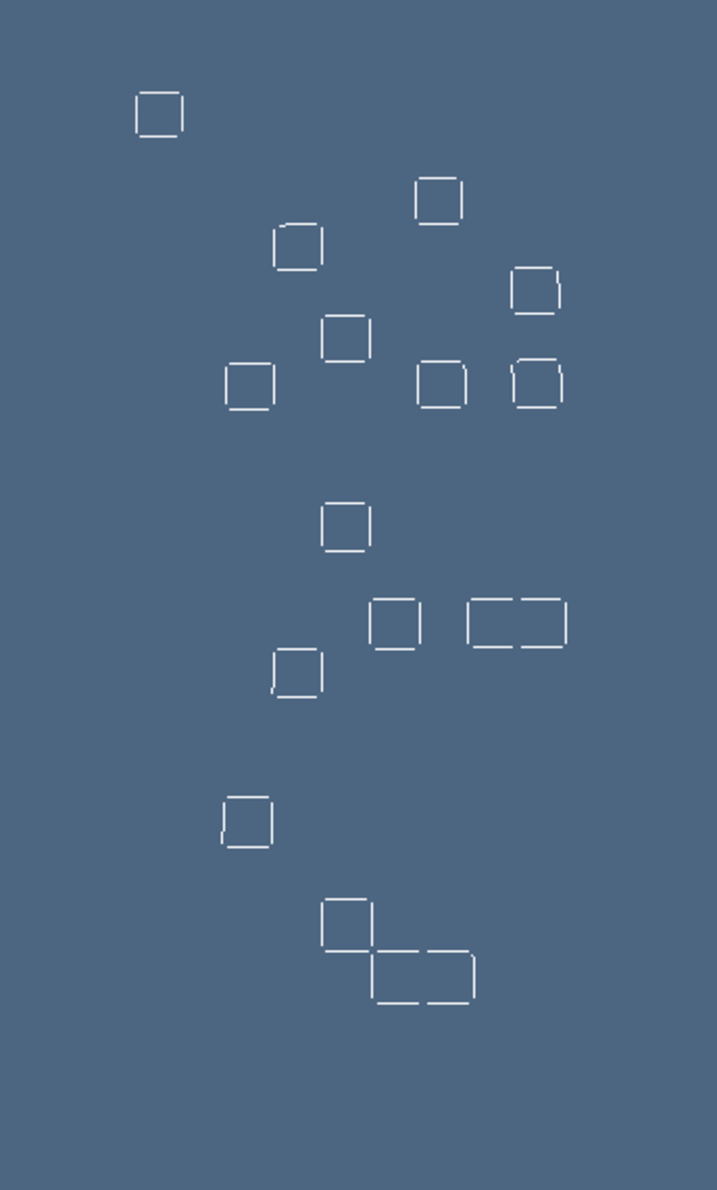
\includegraphics[height=0.3\linewidth,width=0.16\linewidth]{images/morph-chain1D3} 
   \caption{example caption}
   \label{fig:morph}
\end{figure}


\section{Exporting the \texttt{morph} module}

\paragraph{Exporting the morph module}
%-------------------------------------------------------------------------------
@o lib/py/morph.py
@{""" LAR implementation of morphological operators on multidimensional images."""
@< Initial import of modules @>
@< Generation of random image @>
@< Generation of a masking window @>
@< Pyplasm visualisation of an image chain @>
@< Boundary visualisation of an image chain @>
@}
%-------------------------------------------------------------------------------

%-------------------------------------------------------------------------------
@d Initial import of modules
@{
import scipy.misc, numpy
from numpy.random import randint
from pyplasm import *

""" import modules from larcc/lib """
import sys
sys.path.insert(0, 'lib/py/')

@< Import the module @(largrid@) @>
@< Import the module @(morph@) @> 
@}
%-------------------------------------------------------------------------------


\section{Morphological operations examples}

\subsection{2D image masking and boundary computation}

\paragraph{Test example}

The \texttt{larcc.morph} API is used here to generate a random black and white image, with an \emph{image segment} selected and extracted by masking, then colored in middle grey, and exported to an image file.  

%------------------------------------------------------------------
@o test/py/morph/test01.py
@{@< Initial import of modules @>
rows, columns = 100,100
rowSize, columnSize = 10,10
shape = (rows, columns)
structure = (rowSize, columnSize)
image_array = randomImage(shape, structure, 0.3)
minPoint, maxPoint = (20,20), (40,30)
window = minPoint, maxPoint
segmentChain = setMaskWindow(window,image_array)
	
if __name__== "__main__":
	model = visImageChain (shape,segmentChain)
	VIEW(EXPLODE(1.2,1.2,1.2)(MKPOLS(model)))
	model = visImageChainBoundary (shape,segmentChain)
	VIEW(EXPLODE(1.2,1.2,1.2)(MKPOLS(model)))
@}
%------------------------------------------------------------------



%===============================================================================
\appendix
\section{Utilities}

\subsection{Importing a generic module}
First we define a parametric macro to allow the importing of \texttt{larcc} modules from the project repository \texttt{lib/py/}. When the user needs to import some project's module, she may call this macro as done in Section~\ref{sec:lar2psm}.
%------------------------------------------------------------------
@d Import the module
@{import @1
from @1 import *
@}
%------------------------------------------------------------------

\paragraph{Importing a module} A function used to import a generic \texttt{lacccc} module within the current environment is also useful.
%------------------------------------------------------------------
@d Function to import a generic module
@{def importModule(moduleName):
	@< Import the module @(moduleName@) @>
@| importModule @}
%------------------------------------------------------------------


\bibliographystyle{amsalpha}
\bibliography{morph}

\end{document}
